\lab{Random Forests}{Random Forests}
\objective{Understand how to build and use a classification tree and a random forest.}

\section*{Classification Trees} %-----------------------------
Decision
Classification trees are a class of decision trees used in a wide variety of settings where labeled training data is available.
The desired outcome is a model that can accurately assign labels to unlabeled data.
Decision trees are widely used because they have a fast run time, low computation cost, and can handle irrelevant, missing, and noisy data easily.

We begin with a dataset of samples, such as information about customers from a certain store.
Each sample contains a variety of features, such as if the individual is married or has children.
The sample also has a classification label, such as whether or not the person made a specific purchase.

A classification tree is composed of many \emph{nodes}, which ask a question (i.e. ``Is income $\geq$ 85?'') and then split the data based on the answers.
If the response is \texttt{True}, then the sample is ``pushed'' down the tree to the left child node. If the response is \texttt{False}, then the sample is ``pushed'' down the tree to the right child node.
A \emph{leaf} node is a node that has no child node.
Upon arrival at a leaf, an unlabeled sample is labeled with the classification that matches the majority of labeled samples at that leaf.

Table \ref{table:customer-data} includes information about 10 individuals and an indicator of whether or not they made a certain purchase.
To simplify construction of the tree, all data is numeric, so 1=Yes and 0=No for yes/no questions.

Suppose we wanted to guess whether a single college student making under \$30,000 would purchase this item.
Starting at the top of the tree, we compare our sample to the question and first choose the right branch, and then we compare with the second question and choose the right branch again.
Now we reach a leaf with the dictionary \li{\{0:1\}}.
The key \li0 corresponds to the label, and the value \li1 means one of our original samples is at this leaf with that label.
Since 100\% of samples at this leaf are labeled with \li0, our new sample college student will be predicted to share the label \li0.

If we arrived instead at a leaf with the dictionary \li{\{0:1, 1:4\}}, then one of our original samples at this leaf would be labeled \li0 and four would be labeled \li1, so the majority vote would assign the label \li1 to our new sample.

\begin{table}[H]
\begin{center}
\begin{tabular}{c|c|c|c}
Married (Y/N) & Children & Income (\$1000) & Purchased (Y/N) \\ \hline
0 & 5 & 125 & 0 \\
1 & 0 & 100 & 0 \\
0 & 0 & 70 & 0 \\
1 & 3 & 120 & 0 \\
0 & 0 & 95 & 1 \\
1 & 0 & 60 & 0 \\
0 & 2 & 220 & 1 \\
0 & 0 & 85 & 1 \\
1 & 0 & 75 & 0 \\
0 & 0 & 90 & 1
\end{tabular}
\caption{Customer data with 3 features (Married, Children, Income) and a label (Purchase) indicating whether or not the customer bought the item.}
\label{table:customer-data}
\end{center}
\end{table}

\begin{figure}[H]
\centering
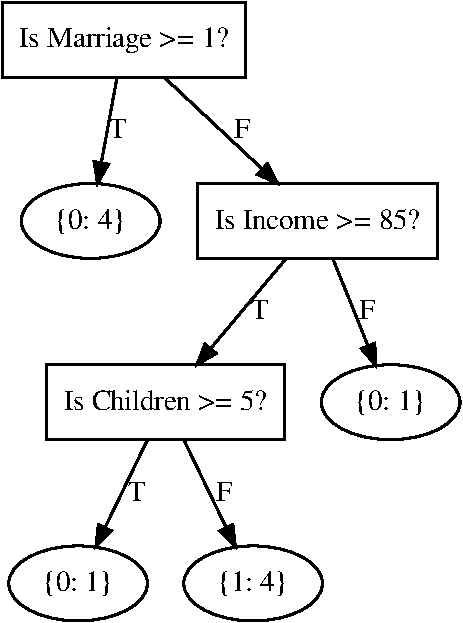
\includegraphics[scale=.8]{example_tree.pdf}
\caption{A classification tree built using Table \ref{table:customer-data}.
Each leaf includes a dictionary of the label (0 or 1) and how many individuals from the data match the classification.
In this example, each leaf contains individuals with only one label.}
\label{figure:simple-tree}
\end{figure}

\begin{problem} %Problem 1
At each node in a classification tree, a question determines which branch a sample belongs to.
The \li{Question} class has attributes \li{column} and \li{value}.
Write a \li{match} method for the \li{Question} class that accepts a sample and returns either \texttt{True} or \texttt{False}.
A sample will be in the form of an array, so in the example above, a single college student with no children making \$20,000 would be represented by the array $[0,0,20]$.
The method should determine if the sample's feature located at index \li{column} is greater than or equal to \li{value}.
Notice that this method will only handle one feature of one sample at a time.

Next, write a \li{partition()} function that partitions the samples (rows) of a dataset for a given \li{Question} into two \li{numpy} arrays, \li{left} and \li{right}, returned in that order.
The array \li{left} will contain the samples that the \li{match} method returned as \texttt{True}, and the array \li{right} will contain the samples that the \li{match} method returned as \texttt{False}.
If \li{left} or \li{right} is empty, still return them as (2-D size zero) arrays.

Hint: if \li{n} is the length of each sample, \li{left.reshape(-1,n)} (and similar for \li{right}) will make the final arrays the correct size even if they're empty.

The file \li{animals.csv} contains information about 7 features for 100 animals.
The last column, the class labels, indicates whether or not an animal lives in the ocean.
You may use this file to test your functions.

\begin{lstlisting}
>>> import numpy as np
# Load in the data
>>> animals = np.loadtxt('animals.csv', delimiter=',')
# Load in feature names
>>> features = np.loadtxt('animal_features.csv', delimiter=',', dtype=str, 
...					comments=None)
# Load in sample names
>>> names = np.loadtxt('animal_names.csv', delimiter=',', dtype=str)

# initialize question and test partition function
>>> question = Question(column=1, value=3, feature_names=features)
>>> left, right = partition(animals, question)
>>> print(len(left), len(right))
62 38

>>> question = Question(column=1, value=75, feature_names=features)
>>> left, right = partition(animals, question)
>>> print(len(left), len(right))
0 100
\end{lstlisting}

\label{prob:1}
\end{problem}


\subsection*{Optimal Split}
To use the \li{partition()} function from Problem \ref{prob:1}, we need to know which question to ask at each node. 
Usually, the question is determined by the split that maximizes either the Gini impurity or the information gain (which itself uses the Gini impurity).
For this lab, we will use the information gain.

Gini impurity measures how often a sample would be mislabeled based on the distribution of labels.
It is a measure of homogeneity of labels, so it is $0$ when all samples at a node have the same label.

\begin{definition}
Let $D$ be a dataset with $K$ different class labels and $N$ different samples.
Let $N_{k}$ be the number of samples labeled class $k$ for each $1 \leq k \leq K$.
We define the \emph{Gini impurity} to be 
\begin{equation*}
G(D) = 1 - \sum_{k=1}^{K} \left(\frac{N_k}{N}\right)^2.
\end{equation*}
\end{definition}

Information gain is based on the concept of information theory entropy.
It measures the difference between two probability distributions.
If the distributions are equal, then the information gain is $0$.
We will use a modified version of information gain for simplicity:

\begin{definition}
Let $s_{D}(p,x) = D_{1},D_{2}$ be a partition of data $D$.
We define the \emph{information gain} of this partition to be 
\begin{equation*}
I(s_{D}(p,x)) = G(D) - \sum_{i=1}^{2} \frac{\abs{D_{i}}}{\abs{D}} \cdot G(D_{i})
\end{equation*}
where $\abs{D}$ represents the number of samples (or rows) in $D$.
\end{definition}

\begin{comment} %this used to be problem 2
\begin{problem}
Write a function \li{gini()} that computes the Gini impurity of a given dataset with the class labels in the last column.
Write another function \li{info_gain()} that computes the information gain for a given split of data.

\noindent Hint: the functions \li{num_rows()} and \li{class_counts()} are provided, which return the number of rows in a given array and a dictionary with the number of samples for each class label, respectively. 

\begin{lstlisting}
# Test your functions
>>> gini(animals)
0.4758
# split animals into two sets with fifty animals in each
>>> info_gain(animals[:50], animals[50:], gini(animals))
0.14579999999999999
\end{lstlisting}
\end{problem}
\end{comment}
The provided function \li{info_gain()} can be used to compute the information gain of a partiton of a dataset.
The optimal split of data at a node can be chosen by finding the question whose partition maximizes the information gain.

Sometimes the partition to split on may separate the data into very small subsets with only a few samples each.
This can make the classification tree vulnerable to overfitting and noisy data.
For this reason, we will include an argument to specify the smallest allowable leaf size, or the minimum number of samples at any node.
A reasonable minimum number depends on the size of the whole dataset, so a dataset with 10,000 samples would have a larger minimum leaf size than our first example with only 10 samples.

To find the optimal split, begin by instantiating \li{best_gain} to 0 and \li{best_question} to \li{None}.
For each unique value in each feature (column) of the dataset, instantiate a \li{Question} object with the column and value, then use \li{partition()} to split the dataset into left and right partitions.
If either the left or right partition has fewer samples than the smallest allowable leaf size (called \mbox{\li{min_samples_leaf}),} then discard this split and iterate to the next one.
If the left and right partitions are ok, then calculate the \li{info_gain()} of these two partitions.
If this \li{info_gain()} is greater than \li{best_gain}, then set \li{best_gain} and \li{best_question} equal to \li{info_gain()} and the corresponding \li{Question}, respectively.
After checking all possible partitions (every column and row), return \li{best_gain} and \li{best_question}.

\begin{problem}
Write a function \li{find\_best\_split()} that computes the optimal split of a dataset by following the directions given above.
Recall that the final column of the dataset contains the class labels, which has no questions associated with it, so do not iterate through the final column.
Include a minimum leaf size argument \li{min_samples_leaf} defaulting to 5.

Return the information gain and corresponding question for the best split, in that order.
If two splits have the same information gain, choose the first split.
Iterate through each feature (column) of the dataset, then through each unique value (row) that the feature takes on; that is, iterate through columns in the outer loop and rows in the inner loop.
If no partitions are possible due to \li{2*min_samples_leaf}, return \li{None} for the question.

\noindent You should get the following output for the animals dataset.
\begin{lstlisting}[mathescape=true]
# Test your function
>>> find_best_split(animals, features)
(0.12259833679833687, Is $\#$ legs/tentacles >= 2.0?)
\end{lstlisting}
\end{problem}

\subsection*{Building the Tree}
Once the optimal split for a node is determined, the node needs to be defined as either a Leaf node or a Decision node. 
As described earlier, leaf nodes have no children, and the classification of samples are determined in leaf nodes.
If the optimal split returns a left and right tree, then the node is a decision node and has a question associated with it to determine which path a sample should follow.
The next two problems will walk through building a classification tree using the functions and classes from the previous problems.

\begin{problem}
The class \li{Leaf} is instantiated with data containing samples in that leaf. 
In the constructor, save an attribute \li{prediction} as a dictionary of how many samples in the leaf belong to each unique class label.

\noindent Hint: remember the provided function \li{class_counts()}.

Write the class \li{Decision_Node}.
This class should have three attributes: an associated \li{Question}, a left branch, and a right branch.
The branches will be \li{Leaf} or \li{Decision_Node} objects.
Name these three attributes \li{question}, \li{left}, and \li{right}.
\end{problem}

In addition to having a minimum leaf size, it's also important to have a maximum depth for trees.
Without restricting the depth, the tree can become very large; if there is no minimum leaf size, it can be one less than the number of training samples.
Limiting the depth can stop the tree from having too many splits, preventing it from becoming too complex and overfitting the training data. 
On the other hand, it's also important to not have too shallow of a tree because then the tree will underfit the data.

\begin{problem}
Write a function \li{build_tree()} that uses your previous functions to build a classification tree.
Include a minimum leaf argument defaulting to 5 and a maximum depth argument defaulting to 4.
Start counting depth at 0.
For comparison, the tree in Figure \ref{figure:simple-tree} has depth 3.
We will build this tree recursively as follows:

\begin{itemize}
\item If the number of samples (rows) in the given data is less than twice \li{min_samples_leaf} (i.e., it can't be split again), then return the data as a \li{Leaf} and that's it.
\item
Otherwise, the data can be split, so find the optimal gain and corresponding question using the function \li{find_best_split()}.
\item
If the optimal gain is 0 (i.e., if the partition is already optimal), or if \li{current_depth} is greater than or equal to \li{max_depth} (i.e., the tree is already too deep), return the data as a \li{Leaf} and that's it.

\item
If the node isn't a \li{Leaf}, then it must be a \li{Decision_Node}.
\begin{itemize}
\item Use \li{partition()} to split the data into left and right partitions.
\item Next, recursively define the right branch and left branch of the tree by calling \li{build_tree()} on each of the left and right partitions with \li{current_depth} incremented by 1.
\item Finally, return a \li{Decision_Node} object using the optimal question found earlier and the left and right branches of the tree.
\end{itemize}
\end{itemize}

The function \li{draw_tree()} is provided to allow you to save a pdf image to view a specified trained tree.
In order to use this function, you must successfully install the \li{graphiz} package.

\li{graphviz} has two parts: an external program, and a Python package that interfaces with that program.
To install both of these parts, refer to the section in Additional Materials.
(Both of these are installed by \li{install_dependencies.sh}.)

With \li{graphviz} installed, you can test your \li{build_tree} function as follows:
\begin{lstlisting}
>>> my_tree = build_tree(animals, features)
>>> draw_tree(my_tree)
\end{lstlisting}
The resulting tree should have 8 question nodes, 9 leaf nodes, and a total of 5 rows of nodes (including the lowermost leaves).
If \li{draw_tree} returns an error about pdf being an unrecognized file type, try running the command \li{dot -c} in your terminal.
\end{problem}

\subsection*{Predicting}
It's important to test your tree to ensure that it predicts class labels fairly accurately and so that you can adjust the minimum leaf and maximum depth parameters as needed.
It is customary to randomly assign some of your labeled data to a training set that you use to fit your tree and then use the rest of your data as a testing set to check accuracy.
%How much to say here?

\begin{problem}
Write a function \li{predict_tree()} that returns the predicted class label for a single new sample given a trained tree called \li{my_tree}.
This function will be implemented recursively in order to traverse the branches and reach a \li{Leaf} node.
Use the \li{isinstance()} function to determine if the current node (\li{my_tree}) is of type \li{Leaf}; if it is, return the label that corresponds with the most samples in the \li{Leaf}.

If the given tree is not a \li{Leaf}, then it is a \li{Decision_Node} with left and right children nodes.
If the \li{my_tree.question.match} method is \texttt{True} with the given sample, then recursively call \li{predict_tree()} with \li{my_tree.left}.
Otherwise, recursively call \li{predict_tree()} with \li{my_tree.right}.

\noindent Hint: an easy way to get the most common value at a \li{Leaf} node is to call \li{max()} on \li{my_tree.prediction} using the keyword argument \li{key=my_tree.prediction.get}.
Remember to return something from both branches of your function.

Next, write a function \li{analyze_tree()} that accepts a labeled dataset (with the labels in the last column, as in \li{animals.csv}) and a trained classification tree.
The function should compare the actual label of each sample (row) with its predicted label using \li{predict_tree()}, and it should return the proportion of samples that the tree labels correctly.

Test your function with the \li{animals.csv} file.
Shuffle the dataset with \li{np.random.shuffle()} and use 80 samples to train your classification tree.
Use the other 20 samples as the test set to see how accurately your tree classifies them.
Your tree should be able to classify this set with roughly 80\% accuracy on average, given the default parameters.
\end{problem}

\section*{Random Forest} %-----------------------------
As noted, one of the main issues with Decision Trees is their tendency to overfit.
Random forests are a way of mitigating overfitting that cannot be fixed by restricting the tree depth and leaf size.
A \emph{random forest} is just what it sounds like--a collection of trees.
Each tree is trained randomly, meaning that at each node, only a small, randomly-chosen subset of the features is available to determine the next split.
The size of this subset should be small relative to the total number of features present.
Let $n$ be the total number of features in the dataset.
A common method which we will use here is to split on $\sqrt{n}$ features (rounding down where applicable).

When predicting the label of a new sample, each trained tree in the forest casts a vote, determined as above, and the sample is labeled according to the majority vote of the trees.

\begin{problem}
Add an argument \li{random_subset} to \li{find_best_split()} and \li{build_tree()}, defaulting to \texttt{False}, that indicates whether or not the tree should be trained randomly.
When \texttt{True}, each node should be restricted to a random combination of $\sqrt{n}$ (rounded down) features to use in its split, where $n$ is the total number of features (note that class labels are not features).
This will require the function \li{find_best_split()} to be altered so that it only iterates through a random combination of $\sqrt{n}$ features (columns).

Next, write a function \li{predict_forest()} that accepts a new sample and a trained forest (as a list of trees).
It should iterate through each tree, finding the label assigned to the sample by calling \li{predict_tree()}.
Then, it should return the label predicted by the majority of the trees.

Finally, write a function \li{analyze_forest()} that accepts a labeled dataset (with the labels in the last column, as in \li{animals.csv}) and a trained forest.
The function should compare the actual label of each sample (row) with its predicted label using \li{predict_forest()}, and it should return the accuracy of the forest's predictions.

Test your functions on the \li{animals.csv} dataset.
Visualize your trees using \li{draw_tree()}, verifying that they are different every time.
Compare the results to the non-randomized version.
\end{problem}

\subsection*{Scikit-Learn}

Finally, we'll compare our implementation to scikit-learn's \li{RandomForestClassifier}.
Rather than accepting all the data as a single array, as in our implementation, this package accepts the feature data as the first argument and all of the labels as the second argument.

\begin{lstlisting}
>>> from sklearn.ensemble import RandomForestClassifier

# Create the forest with the appropriate arguments and 200 trees
>>> forest = RandomForestClassifier(n_estimators=200, max_depth=4,
...									min_samples_leaf=5)

# Shuffle the data
>>> shuffled = np.random.permutation(animals)
>>> train = shuffled[:80]
>>> test = shuffled[80:]

# Fit the model to your data, passing the labels in as the second argument
>>> forest.fit(train[:,:-1], train[:,-1])

# Test the accuracy with the testing set
>>> forest.score(test[:,:-1], test[:,-1])
0.85
\end{lstlisting}

\begin{problem}
The file \li{parkinsons.csv} contains annotated speech data from people with and without Parkinson's Disease.
The first column is the subject ID, columns 2-27 are various features, and the last column is the label indicating whether or not the subject has Parkinson's. 
You will need to remove the first column so your forest doesn't use participant ID to predict class labels.
Feature names are contained in the file \li{parkinsons_features.csv}.

Write a function to compare your forest implementation to the package from scikit-learn.
Because of the size of this dataset, we will only use a small portion of the samples and build a very simple forest.
Randomly select 130 samples.
Use 100 in training your forest and 30 more in testing it.
Build 5 trees for your forest (as a list) using \li{min_samples_leaf=15} and \li{max_depth=4} for each tree.
Time how long it takes to train and analyze your forest.

Repeat this with scikit-learn's package, using the same 100 training samples and 30 test samples.
Set \li{n_estimators=5}, \li{min_samples_leaf=15}, and \li{max_depth=4}.

Then, using scikit-learn's package, run the whole \li{parkinsons.csv} dataset, using the default parameters.
Use 80\% of the data to train the forest and the other 20\% to test it.

Return three tuples: the accuracy and time of your implementation, the accuracy and time of scikit-learn's package, and then the accuracy and time of scikit-learn's package using the entire dataset.
\end{problem}

\section*{Additional Materials}
\subsection*{Installing Graphviz}
The Python package can be installed using \li{pip install graphviz}.
To install the external program,
on Windows in the WSL terminal and on Linux use the following:
\begin{lstlisting}
sudo apt-get install graphviz
\end{lstlisting}
On Mac:
\begin{lstlisting}
brew install graphviz
\end{lstlisting}
For additional options for the external program, refer to the instructions at \url{https://graphviz.org/download/}.
